\documentclass[a4paper,11pt]{article}
\usepackage[utf8]{inputenc}
\usepackage{geometry}
\usepackage{xcolor}
\usepackage{hyperref}
\usepackage{amsmath}
\usepackage{amssymb}
\usepackage{tcolorbox}
\usepackage{booktabs}
\usepackage{array}
\usepackage{tikz}

% Page geometry (tighter than the online guides: bench budget of 3 + 2 pages)
\geometry{top=1.8cm, bottom=1.8cm, left=2cm, right=2cm}
\hypersetup{pdftitle={Lab 9: BB84 on the Bench}, colorlinks=true, linkcolor=ibmblue, urlcolor=ibmblue}
\pagestyle{plain}
\setlength{\parindent}{0pt}
\setlength{\parskip}{3pt}

% Custom colours
\definecolor{ibmblue}{RGB}{0, 45, 156}
\definecolor{ibmred}{RGB}{250, 75, 76}
\definecolor{purpleaccent}{RGB}{109, 40, 217}
\definecolor{amberaccent}{RGB}{245, 158, 11}
\definecolor{tealaccent}{RGB}{13, 148, 136}
\definecolor{shockorange}{RGB}{234, 88, 12}

% Custom boxes (titles always in braced form)
\newtcolorbox{studentbox}{colback=blue!5!white,colframe=blue!75!black,title={Student Activity}}
\newtcolorbox{theorybox}{colback=gray!5!white,colframe=gray!50!black,title={Theory Recap}}
\newtcolorbox{warningbox}{colback=yellow!10!white,colframe=orange!80!black,title={Important}}
\newtcolorbox{simulatorbox}{colback=purple!5!white,colframe=purple!75!black,title={Simulator}}
\newtcolorbox{reflectionbox}{colback=teal!5!white,colframe=teal!75!black,title={Quick Check}}
\newtcolorbox{connectionbox}{colback=green!5!white,colframe=green!60!black,title={Connections to Previous Labs}}
\newtcolorbox{procedurebox}{colback=red!4!white,colframe=red!70!black,title={Procedure 1 vs Procedure 2}}
\newtcolorbox{questionbox}{colback=violet!4!white,colframe=violet!70!black,title={The Question}}
\newtcolorbox{shockbox}{colback=shockorange!8!white,colframe=shockorange,title={Counterintuitive --- and Real}}
\newtcolorbox{benchbox}{colback=teal!6!white,colframe=tealaccent,title={Open the Simulator First}}
\newtcolorbox{numberbox}{colback=green!4!white,colframe=green!50!black,title={Formula $\rightarrow$ Number $\rightarrow$ Bench}}
\newtcolorbox{industrybox}{colback=amberaccent!10!white,colframe=amberaccent!90!black,title={Real-World Anchor}}
\newtcolorbox{deepdivebox}{colback=cyan!4!white,colframe=cyan!60!black,title={Deep Dive}}

% Titled variants for this guide (same colour schemes as above)
\newtcolorbox{devbox}[1]{colback=yellow!10!white,colframe=orange!80!black,title={#1}}
\newtcolorbox{labelbox}[1]{colback=gray!5!white,colframe=gray!50!black,title={#1}}
\newtcolorbox{demobox}[1]{colback=cyan!4!white,colframe=cyan!60!black,title={#1}}
\newtcolorbox{pmcbox}[1]{colback=blue!5!white,colframe=blue!75!black,title={#1}}

% Compact spacing for every box (look unchanged)
\tcbset{left=4pt, right=4pt, top=2pt, bottom=2pt, boxsep=2pt,
        before skip=5pt, after skip=5pt, fonttitle=\bfseries\small}

% Bra-ket shorthands (guarded: never clash with package-provided macros)
\providecommand{\ket}[1]{|#1\rangle}
\providecommand{\bra}[1]{\langle#1|}
\providecommand{\braket}[2]{\langle#1|#2\rangle}

% Section headings: each Part heading is its question
\makeatletter
\renewcommand\section{\@startsection{section}{1}{\z@}{-1.6ex \@plus -.5ex}{0.6ex}{\normalfont\large\bfseries\color{ibmblue}}}
\makeatother

% Compact lists (no enumitem)
\newenvironment{steps}{\begin{enumerate}\setlength{\itemsep}{1pt}\setlength{\parsep}{0pt}\setlength{\topsep}{2pt}}{\end{enumerate}}

% Worksheet cells
\newcolumntype{L}{>{\rule[-1.7mm]{0pt}{5.4mm}\footnotesize\raggedright\arraybackslash}p{2.75cm}}
\newcolumntype{C}{>{\centering\arraybackslash\scriptsize}p{0.62cm}}
\newcolumntype{K}{>{\rule[-1.7mm]{0pt}{5.4mm}\centering\arraybackslash\scriptsize}p{0.54cm}}
\newcommand{\blank}[1]{\rule{#1}{0.4pt}}

\begin{document}

% =====================================================================
% === Header ===
% =====================================================================
{\LARGE\bfseries\color{ibmblue} Lab 9: BB84 on the Bench}\par
\vspace{2pt}
{\large Quantum key distribution (QKD) on a tabletop kit}\hfill
\textbf{1 ECTS}\,$\cdot$\,in person at i-LAMP\par
\vspace{4pt}
\textbf{Prerequisites:} \textit{Fundamental Concepts of Quantum Technologies} and
\textit{Quantum Communication} (lecture series) --- nothing else.\\
\textbf{What you need:} the Thorlabs EDU-QCRY1 kit with Alice, Bob and Eve modules
(set up by the staff); Alice's black 8-sided die, red 6-sided dice for Bob and Eve; the
worksheet (pages 4--5); a pen.\\
\textbf{Safety:} class 2 laser, 635\,nm, pulses of at most 1\,mW. Never stare into the
beam or its reflections; if dazzled, close your eyes and turn away (manual Ch.~13).\\
{\footnotesize\textbf{Source:} Thorlabs, \textit{EDU-QCRY1 Quantum Cryptography Demonstration Kit User
Manual}, Rev~D (2026), ``manual \S x''.}\\
\textbf{Goal:} run BB84, the QKD protocol of the \textit{Quantum Communication} course, on
an optical bench, and find out what the bench can and cannot show.

\begin{center}
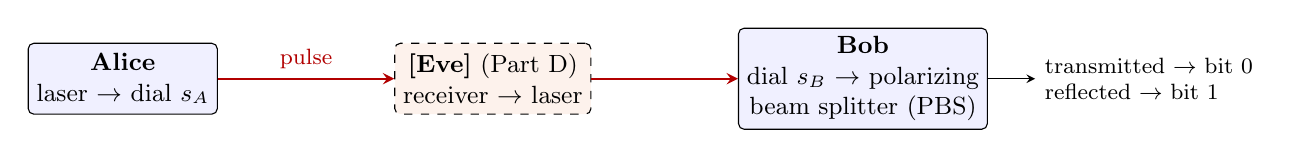
\begin{tikzpicture}[font=\small, >=stealth,
  mod/.style={draw, rounded corners=2pt, align=center, minimum height=9mm, inner sep=3pt}]
  \node[mod, fill=blue!6] (A) at (0,0) {\textbf{Alice}\\ laser $\to$ dial $s_A$};
  \node[mod, dashed, fill=shockorange!8] (E) at (4.7,0) {\textbf{[Eve]} (Part D)\\ receiver $\to$ laser};
  \node[mod, fill=blue!6] (B) at (9.4,0) {\textbf{Bob}\\ dial $s_B$ $\to$ polarizing\\ beam splitter (PBS)};
  \node[font=\footnotesize, align=left, anchor=west, xshift=6mm] (S) at (B.east) {transmitted $\to$ bit 0\\ reflected $\to$ bit 1};
  \draw[->, thick, red!70!black] (A) -- node[above, font=\footnotesize]{pulse} (E);
  \draw[->, thick, red!70!black] (E) -- (B);
  \draw[->] (B) -- (S);
\end{tikzpicture}
\end{center}

% =====================================================================
% === Part A ===
% =====================================================================
\section*{Part A --- Does the channel work?}

\textbf{Intuition.} Alice's laser emits horizontally polarized pulses. In Dirac notation (from
\textit{Fundamental Concepts}) we call horizontal polarization $\ket{H}$ and vertical $\ket{V}$, and use them as the bits: $\ket{H}
\leftrightarrow 0$, $\ket{V} \leftrightarrow 1$. Light polarized at angle $\theta$
(from the horizontal, counter-clockwise as seen from behind Alice's laser, looking along
the beam) is $\ket{\theta} = \cos\theta\,\ket{H} + \sin\theta\,\ket{V}$. A
\textbf{basis} here is a pair of perpendicular polarizations: the $+$ basis
$\{0^\circ, 90^\circ\}$ and the $\times$ basis $\{-45^\circ, 45^\circ\}$.

\textbf{The half-wave-plate rule.} A half-wave plate mirrors the polarization direction
about the plate's axis; each module's dial reads the result directly in polarization
degrees (the dial shows twice the axis angle). \emph{Alice's dial turns horizontal light
to the dial angle:} her axis sits at $s_A/2$ and mirrors $0^\circ$ to $s_A$, so her
pulse leaves as $\ket{s_A}$. \emph{Bob's dial faces the other way} (away from Alice, manual \S7.4),
so it reads with the opposite sign: his axis sits at $-s_B/2$ and mirrors $\ket{s_A}$
to $\ket{-s_B - s_A} = \ket{-(s_A+s_B)}$, and that is the light reaching his PBS.

\textbf{Formula.} The polarizing beam splitter (PBS) transmits $\ket{H}$ to one
sensor (bit 0) and reflects $\ket{V}$ to the other (bit 1). The Born rule (\textit{Fundamental Concepts}) gives
$P(\text{transmitted}) = |\braket{H}{\theta'}|^2 = \cos^2\theta'$ for light at angle
$\theta'$; for a bright beam this is Malus's law, the transmitted fraction of the
intensity. With $\theta' = -(s_A + s_B)$:
\begin{equation*}
  P(\text{transmitted}) = \cos^2(s_A + s_B), \qquad P(\text{reflected}) = \sin^2(s_A + s_B).
\end{equation*}
Bob measures in two steps: his plate maps the basis he chose onto the $H/V$ split, then
the PBS splits it and the sensor absorbs the light.
\textbf{Number:} $s_A = 45^\circ$, $s_B = 45^\circ$ gives $\cos^2 90^\circ = 0$:
reflected, bit 1.

\begin{pmcbox}{Predict $\rightarrow$ measure $\rightarrow$ compare (worksheet W1)}
\begin{steps}
  \item \textbf{Predict} all 8 cases, $s_A \in \{-45^\circ, 0^\circ, 45^\circ, 90^\circ\}$
        and $s_B \in \{0^\circ, 45^\circ\}$: transmitted (T), reflected (R), or
        \emph{both} where the formula gives $\tfrac12$.
  \item \textbf{Measure} in \emph{adjustment mode} (yellow side LED: when both sensors
        receive equal light, both blue LEDs light; manual \S7.2.3). Check the alignment
        with the fine-tuning steps of manual \S7.4, then fire one pulse per case.
  \item \textbf{Compare.} All 8 cases must match before Part C. If one fails, call the
        staff (troubleshooting: manual Ch.~11).
\end{steps}
\end{pmcbox}

% DEV-9.3: no loss or noise model; misalignment appears as QBER without Eve
\begin{devbox}{The bench is not the model: misalignment}
Our formula assumes perfect plates, dials and sensors, with no loss and no noise. A
plate or sensor slightly off moves a ``certain'' case away from exactly 0 or 1, so some
pulses light the wrong LED. In Part C this shows up as \emph{errors without any Eve}.
That is why all 8 cases must pass first, and why nobody leans on or moves the table
during a run (manual \S7.4).
\end{devbox}

% =====================================================================
% === Part B ===
% =====================================================================
\section*{Part B --- Who flips the coin?}

In 4 of the 8 cases Alice and Bob use different bases, the formula gives $\tfrac12$, and
in adjustment mode \emph{both} LEDs light. \textbf{Predict:} a real photon would give a
single random bit, 0 or 1 with probability $\tfrac12$ each. \textbf{Measure:} keep one
$\tfrac12$ case, switch to \emph{measuring mode} (green side LED), fire several pulses
and tally T and R in W1. \textbf{Compare} with what adjustment mode showed for the same
settings.

% DEV-9.1: bright pulses + electronic coin instead of single photons + quantum randomness
\begin{shockbox}
The pulse is classical light: at a $\tfrac12$ case it really \emph{does} split, half the
intensity to each sensor --- that is what adjustment mode shows. In measuring mode the
kit's electronics \textbf{picks one LED at random} (manual \S7.2.3). A single photon
would not split: it reaches one sensor or the other, and nothing on the bench decides in
advance which. The statistics are the same Born numbers, but here the coin is
electronic. \textbf{The kit is an analogy of BB84}, not a quantum channel.
\end{shockbox}

% =====================================================================
% === Part C ===
% =====================================================================
\section*{Part C --- Can Alice and Bob agree on a secret?}

\textbf{Intuition.} When Alice's and Bob's bases match, Bob's bit equals Alice's (Part
A); when they differ, Bob's bit is a coin flip. So they keep only the matched pulses,
and they can find those by talking in public without ever saying a bit.
\begin{steps}
  \item \textbf{Dice, before firing.} For each of $N = 52$ pulses, Alice rolls the
        8-sided die (each face shows a basis and a bit) and Bob the 6-sided die (each
        face shows a basis) (manual Ch.~10). Fill rows 1--3 of W2. Use the dice, not
        your head: people are poor random number generators.
  \item \textbf{Transmit} in measuring mode. Alice sets $+$: $0^\circ$ for 0,
        $90^\circ$ for 1; $\times$: $-45^\circ$ for 0, $45^\circ$ for 1. Bob sets
        $0^\circ$ for $+$ and $45^\circ$ for $\times$, and records transmitted = 0,
        reflected = 1.
  \item \textbf{Sift.} \emph{Sifting} means keeping only the pulses where Alice's and
        Bob's bases agree. They read out their bases in public (never their bits) and
        tick ``same basis''. The bases match with probability
        $\tfrac12\cdot\tfrac12 + \tfrac12\cdot\tfrac12 = \tfrac12$, so the sifted length
        $S$ is about $N/2 = 26$, and $P(S \ge 20) = 96.5\,\%$.
  \item \textbf{Test.} Publicly compare $t = 6$ sifted bits at random positions, chosen
        after the transmission; mark each one $=$ (same bit) or $\neq$ (different bit) in
        the Test row, and drop them from the key. The \emph{QBER} (quantum bit error rate) is
        the probability that Bob's sifted bit differs from Alice's; its estimate is
        (number of errors)$/t$. Predicted without Eve on an aligned bench: QBER $= 0$.
  \item \textbf{Encrypt --- only if the test shows 0 errors.} The \emph{one-time pad}
        adds each message bit $m$ to a key bit $k$ modulo 2 (XOR:
        $0\oplus0 = 1\oplus1 = 0$, $0\oplus1 = 1\oplus0 = 1$), $y = m \oplus k$, with a
        key as long as the message, random, and used only once. Since $k \oplus k = 0$,
        Bob recovers $(m\oplus k)\oplus k = m$. Code a 4-letter word with the 5-bit
        alphabet (manual Ch.~9; W5): 20 key bits from the untested sifted bits. The
        ciphertext may travel in public (manual \S8.2); Bob decrypts it.
\end{steps}
\textbf{Budget:} 20 key bits $+$ 6 test bits need $S \ge 26$, which 52 pulses give with
probability $55.5\,\%$. If you fall short, fire more pulses (manual \S8.1; W2 has room for pulses 53--70); never reuse
key bits. \emph{This is the BB84 order: sift, test, then encrypt. Manual Ch.~8 encrypts
first, as a first-pass teaching sequence (manual Ch.~10).}

\begin{labelbox}{The $\times$ labels}
In the $\times$ basis, bit 0 is the ``$-45$'' setting on Alice's dial and bit 1 the
``$45$'' setting; Bob's ``$45$'' setting reads transmitted as 0. Which diagonal is called
``0'' is a naming convention with no physical effect: renaming both would change no LED
and no error count.
\end{labelbox}

% =====================================================================
% === Part D ===
% =====================================================================
\section*{Part D --- Can Eve hide?}

\textbf{Intuition.} Eve, the eavesdropper, does \emph{intercept-resend}: she catches each pulse with her own
receiver in a basis from her sheet, then re-sends what she read with her own laser in
that basis (manual \S7.5, \S8.3). She cannot know Alice's basis in advance.
\textbf{Predict} on the sifted pulses: half the time Eve's basis equals Alice's, she
reads Alice's bit and re-sends it exactly (error 0); half the time it differs, her bit
is a coin flip and so is Bob's (error $\tfrac12$):
\begin{equation*}
  Q = \tfrac12\cdot 0 + \tfrac12\cdot\tfrac12 = 25\,\%.
\end{equation*}
\textbf{Measure:} the staff insert Eve (manual \S7.5). Eve fills her basis row in W3 with a red
6-sided die \emph{before} the run, so what she sees cannot bias her choices (manual \S8.3). Repeat
Part C steps 1--4 with fresh dice (run 2, W3). No message is encrypted in run 2, so
\emph{every} sifted bit is a test bit: $t = S$. \textbf{Compare}
your QBER with $25\,\%$, and check whether your errors sit only where Eve's basis
differs from Alice's.

\begin{shockbox}
Each test bit catches Eve with probability $\tfrac14$, so she survives $t$ test bits with
probability $(3/4)^t$. With $t = 6$ that is \textbf{17.8\,\%}. Pushing it below 1\,\% takes $t = 17$ ($(3/4)^{17} \approx 0.75\,\%$). Then
20 key bits $+$ 17 test bits need $S \ge 37$: 52 pulses give that only 0.16\,\% of the
time, while about \textbf{85 pulses} give it with 90\,\% probability.
\end{shockbox}

\textbf{Why pool the class data.} The \emph{standard error} (SE) is the typical size of
the random scatter of an estimate around the true value. For the QBER estimate from $t$
test bits, $\text{SE} = \sqrt{Q(1-Q)/t}$: at $Q = 0.25$ and $t = 6$, SE $\approx 0.18$,
so one group's estimate can land far from $25\,\%$. Testing every sifted bit shrinks it:
at $t = 26$, SE $\approx 0.085$. $G$ groups with $t$ test
bits each give $\sqrt{Q(1-Q)/(G\,t)}$. Add your counts to the class table and compute the
class-pooled QBER: total errors over total test bits.

\begin{industrybox}
The \textbf{Micius} satellite distributed BB84 keys from space to the ground (2017);
\textbf{EuroQCI} is the European Commission's initiative for a quantum communication
infrastructure across the EU. Real QKD needs single photons (or \emph{decoy states}:
randomly varied pulse intensities that expose a tap), because bright classical light
can be tapped.
\end{industrybox}

\begin{demobox}{Instructor demo (Part E, optional)}
A non-polarizing beam splitter (NPBS, not in the kit) between Alice and Bob sends part
of every pulse to Eve's receiver and lets the rest through. Bob's QBER stays 0, yet Eve
learns the sifted bits where her basis matched Alice's --- half of them on average, and
she knows which. A single photon cannot be split, so this attack needs classical light.
\end{demobox}

% =====================================================================
% === Report ===
% =====================================================================
\section*{For your report}
\begin{steps}
  \item Is the class-pooled QBER of run 2 consistent with $25\,\%$ within its standard
        error? Is your run-1 QBER consistent with 0, and if not, what on the bench could
        explain it?
  \item Why may Alice and Bob announce their bases in public but never their bits? What
        does Eve learn from the announcements?
  \item Part B and the tap demo both rely on classical light splitting. What would change
        with a true single-photon source?
  \item Look only at the first 6 sifted bits of run 2: would a 6-bit test have caught Eve?
\end{steps}

% =====================================================================
% === Worksheet ===
% =====================================================================
\newpage
\setlength{\tabcolsep}{2pt}
{\large\bfseries\color{ibmblue} Worksheet --- Lab 9: BB84 on the Bench}\par
{\small Group \blank{1.5cm}\quad Names \blank{8.5cm}\quad Date \blank{2.5cm}}

\vspace{4pt}
\textbf{W1 \,$\cdot$\, Part A: the 8 cases (adjustment mode).}
{\small Predict T, R or both from $\cos^2(s_A+s_B)$, then record what lights up.}\\[2pt]
{\small
\begin{tabular}{|c|c|c|c|c|c|c|}\hline
 & \multicolumn{3}{c|}{$s_B = 0^\circ$} & \multicolumn{3}{c|}{$s_B = 45^\circ$} \\ \hline
$s_A$ & $\cos^2(s_A+s_B)$ & predict & observed & $\cos^2(s_A+s_B)$ & predict & observed \\ \hline
\rule[-1.7mm]{0pt}{5.4mm}$-45^\circ$ & & & & & & \\ \hline
\rule[-1.7mm]{0pt}{5.4mm}$0^\circ$   & & & & & & \\ \hline
\rule[-1.7mm]{0pt}{5.4mm}$45^\circ$  & & & & & & \\ \hline
\rule[-1.7mm]{0pt}{5.4mm}$90^\circ$  & & & & & & \\ \hline
\end{tabular}}\\[3pt]
{\small \textbf{Part B, measuring mode} on one $\tfrac12$ case ($s_A$ = \blank{0.9cm},
$s_B$ = \blank{0.9cm}): T tally \blank{2cm} R tally \blank{2cm}.
What changed from adjustment mode? \blank{4.6cm}}

\vspace{5pt}
\textbf{W2 \,$\cdot$\, Run 1: Alice and Bob, no Eve} {\small ($N = 52$ pulses in blocks
of $18 + 18 + 16$).} {\small Basis: $+$ or $\times$. Bit: 0 or 1 (Bob: transmitted = 0,
reflected = 1). Tick matched bases; in the Test row write $=$ or $\neq$ on each test
bit.}\\[2pt]
\begin{tabular}{|L|*{18}{C|}}\hline
\textbf{Pulse} & 1 & 2 & 3 & 4 & 5 & 6 & 7 & 8 & 9 & 10 & 11 & 12 & 13 & 14 & 15 & 16 & 17 & 18 \\ \hline
Alice basis &  &  &  &  &  &  &  &  &  &  &  &  &  &  &  &  &  &  \\ \hline
Alice bit &  &  &  &  &  &  &  &  &  &  &  &  &  &  &  &  &  &  \\ \hline
Bob basis &  &  &  &  &  &  &  &  &  &  &  &  &  &  &  &  &  &  \\ \hline
Bob bit &  &  &  &  &  &  &  &  &  &  &  &  &  &  &  &  &  &  \\ \hline
Same basis? \checkmark &  &  &  &  &  &  &  &  &  &  &  &  &  &  &  &  &  &  \\ \hline
Test $=$\,/\,$\neq$ &  &  &  &  &  &  &  &  &  &  &  &  &  &  &  &  &  &  \\ \hline
\end{tabular}
\par\smallskip
\begin{tabular}{|L|*{18}{C|}}\hline
\textbf{Pulse} & 19 & 20 & 21 & 22 & 23 & 24 & 25 & 26 & 27 & 28 & 29 & 30 & 31 & 32 & 33 & 34 & 35 & 36 \\ \hline
Alice basis &  &  &  &  &  &  &  &  &  &  &  &  &  &  &  &  &  &  \\ \hline
Alice bit &  &  &  &  &  &  &  &  &  &  &  &  &  &  &  &  &  &  \\ \hline
Bob basis &  &  &  &  &  &  &  &  &  &  &  &  &  &  &  &  &  &  \\ \hline
Bob bit &  &  &  &  &  &  &  &  &  &  &  &  &  &  &  &  &  &  \\ \hline
Same basis? \checkmark &  &  &  &  &  &  &  &  &  &  &  &  &  &  &  &  &  &  \\ \hline
Test $=$\,/\,$\neq$ &  &  &  &  &  &  &  &  &  &  &  &  &  &  &  &  &  &  \\ \hline
\end{tabular}
\par\smallskip
\begin{tabular}{|L|*{16}{C|}}\hline
\textbf{Pulse} & 37 & 38 & 39 & 40 & 41 & 42 & 43 & 44 & 45 & 46 & 47 & 48 & 49 & 50 & 51 & 52 \\ \hline
Alice basis &  &  &  &  &  &  &  &  &  &  &  &  &  &  &  &  \\ \hline
Alice bit &  &  &  &  &  &  &  &  &  &  &  &  &  &  &  &  \\ \hline
Bob basis &  &  &  &  &  &  &  &  &  &  &  &  &  &  &  &  \\ \hline
Bob bit &  &  &  &  &  &  &  &  &  &  &  &  &  &  &  &  \\ \hline
Same basis? \checkmark &  &  &  &  &  &  &  &  &  &  &  &  &  &  &  &  \\ \hline
Test $=$\,/\,$\neq$ &  &  &  &  &  &  &  &  &  &  &  &  &  &  &  &  \\ \hline
\end{tabular}
\par\smallskip
{\small\textbf{Extra pulses 53--70} (only if $S < 26$).}\\[2pt]
\begin{tabular}{|L|*{18}{C|}}\hline
\textbf{Pulse} & 53 & 54 & 55 & 56 & 57 & 58 & 59 & 60 & 61 & 62 & 63 & 64 & 65 & 66 & 67 & 68 & 69 & 70 \\ \hline
Alice basis &  &  &  &  &  &  &  &  &  &  &  &  &  &  &  &  &  &  \\ \hline
Alice bit &  &  &  &  &  &  &  &  &  &  &  &  &  &  &  &  &  &  \\ \hline
Bob basis &  &  &  &  &  &  &  &  &  &  &  &  &  &  &  &  &  &  \\ \hline
Bob bit &  &  &  &  &  &  &  &  &  &  &  &  &  &  &  &  &  &  \\ \hline
Same basis? \checkmark &  &  &  &  &  &  &  &  &  &  &  &  &  &  &  &  &  &  \\ \hline
Test $=$\,/\,$\neq$ &  &  &  &  &  &  &  &  &  &  &  &  &  &  &  &  &  &  \\ \hline
\end{tabular}

% --- worksheet page 2 ---
\newpage
\textbf{W3 \,$\cdot$\, Run 2: with Eve} {\small (Eve's basis row is filled with her die \emph{before}
the run). No encryption in run 2: every matched pulse is a test bit, so write $=$ or
$\neq$ on each one.}\\[2pt]
\begin{tabular}{|L|*{18}{C|}}\hline
\textbf{Pulse} & 1 & 2 & 3 & 4 & 5 & 6 & 7 & 8 & 9 & 10 & 11 & 12 & 13 & 14 & 15 & 16 & 17 & 18 \\ \hline
\textbf{Eve basis} &  &  &  &  &  &  &  &  &  &  &  &  &  &  &  &  &  &  \\ \hline
Alice basis &  &  &  &  &  &  &  &  &  &  &  &  &  &  &  &  &  &  \\ \hline
Alice bit &  &  &  &  &  &  &  &  &  &  &  &  &  &  &  &  &  &  \\ \hline
Bob basis &  &  &  &  &  &  &  &  &  &  &  &  &  &  &  &  &  &  \\ \hline
Bob bit &  &  &  &  &  &  &  &  &  &  &  &  &  &  &  &  &  &  \\ \hline
Same basis? \checkmark &  &  &  &  &  &  &  &  &  &  &  &  &  &  &  &  &  &  \\ \hline
Test $=$\,/\,$\neq$ &  &  &  &  &  &  &  &  &  &  &  &  &  &  &  &  &  &  \\ \hline
\end{tabular}
\par\smallskip
\begin{tabular}{|L|*{18}{C|}}\hline
\textbf{Pulse} & 19 & 20 & 21 & 22 & 23 & 24 & 25 & 26 & 27 & 28 & 29 & 30 & 31 & 32 & 33 & 34 & 35 & 36 \\ \hline
\textbf{Eve basis} &  &  &  &  &  &  &  &  &  &  &  &  &  &  &  &  &  &  \\ \hline
Alice basis &  &  &  &  &  &  &  &  &  &  &  &  &  &  &  &  &  &  \\ \hline
Alice bit &  &  &  &  &  &  &  &  &  &  &  &  &  &  &  &  &  &  \\ \hline
Bob basis &  &  &  &  &  &  &  &  &  &  &  &  &  &  &  &  &  &  \\ \hline
Bob bit &  &  &  &  &  &  &  &  &  &  &  &  &  &  &  &  &  &  \\ \hline
Same basis? \checkmark &  &  &  &  &  &  &  &  &  &  &  &  &  &  &  &  &  &  \\ \hline
Test $=$\,/\,$\neq$ &  &  &  &  &  &  &  &  &  &  &  &  &  &  &  &  &  &  \\ \hline
\end{tabular}
\par\smallskip
\begin{tabular}{|L|*{16}{C|}}\hline
\textbf{Pulse} & 37 & 38 & 39 & 40 & 41 & 42 & 43 & 44 & 45 & 46 & 47 & 48 & 49 & 50 & 51 & 52 \\ \hline
\textbf{Eve basis} &  &  &  &  &  &  &  &  &  &  &  &  &  &  &  &  \\ \hline
Alice basis &  &  &  &  &  &  &  &  &  &  &  &  &  &  &  &  \\ \hline
Alice bit &  &  &  &  &  &  &  &  &  &  &  &  &  &  &  &  \\ \hline
Bob basis &  &  &  &  &  &  &  &  &  &  &  &  &  &  &  &  \\ \hline
Bob bit &  &  &  &  &  &  &  &  &  &  &  &  &  &  &  &  \\ \hline
Same basis? \checkmark &  &  &  &  &  &  &  &  &  &  &  &  &  &  &  &  \\ \hline
Test $=$\,/\,$\neq$ &  &  &  &  &  &  &  &  &  &  &  &  &  &  &  &  \\ \hline
\end{tabular}

\vspace{5pt}
\textbf{W4 \,$\cdot$\, Results.} {\small QBER = errors$/t$ ($t$ = marked Test cells, errors = cells marked $\neq$);\quad SE $= \sqrt{Q(1-Q)/t}$ at $Q = 0.25$;\quad
class QBER = total errors$\,/\,$total test bits of all $G$ groups, pooled SE $= \sqrt{Q(1-Q)/(G\,t)}$.}\\[2pt]
{\small
\begin{tabular}{|l|*{7}{>{\centering\arraybackslash}p{1.3cm}|}>{\centering\arraybackslash}p{2.9cm}|}\hline
 & $S$ & $S/N$ & $t$ & errors & QBER & SE\newline{\scriptsize($Q{=}0.25$)} & $(3/4)^t$ & class QBER $\pm$ pooled SE \\ \hline
\rule[-2mm]{0pt}{6.5mm}Run 1 (no Eve) & & & & & & & & \\ \hline
\rule[-2mm]{0pt}{6.5mm}Run 2 (Eve)    & & & & & & & & \\ \hline
\end{tabular}}

\vspace{5pt}
\textbf{W5 \,$\cdot$\, Encryption} {\small (only if run 1 showed 0 test errors).
Ciphertext $y = m \oplus k$; Bob recovers $m = y \oplus k$.}\\[2pt]
{\small
\begin{tabular}{|L|*{20}{K|}}\hline
Letter & \multicolumn{5}{c|}{} & \multicolumn{5}{c|}{} & \multicolumn{5}{c|}{} & \multicolumn{5}{c|}{} \\ \hline
Message bits $m$ & & & & & & & & & & & & & & & & & & & & \\ \hline
Key bits $k$ & & & & & & & & & & & & & & & & & & & & \\ \hline
Ciphertext $y$ & & & & & & & & & & & & & & & & & & & & \\ \hline
\end{tabular}}\\[4pt]
{\small 5-bit alphabet (manual Ch.~9): letter, index, code.}\\[2pt]
{\footnotesize\setlength{\tabcolsep}{3.2pt}
\begin{tabular}{|*{13}{c|}}\hline
\textbf{A}\,0 & \textbf{B}\,1 & \textbf{C}\,2 & \textbf{D}\,3 & \textbf{E}\,4 & \textbf{F}\,5 & \textbf{G}\,6 & \textbf{H}\,7 & \textbf{I}\,8 & \textbf{J}\,9 & \textbf{K}\,10 & \textbf{L}\,11 & \textbf{M}\,12 \\
\texttt{00000} & \texttt{00001} & \texttt{00010} & \texttt{00011} & \texttt{00100} & \texttt{00101} & \texttt{00110} & \texttt{00111} & \texttt{01000} & \texttt{01001} & \texttt{01010} & \texttt{01011} & \texttt{01100} \\ \hline
\textbf{N}\,13 & \textbf{O}\,14 & \textbf{P}\,15 & \textbf{Q}\,16 & \textbf{R}\,17 & \textbf{S}\,18 & \textbf{T}\,19 & \textbf{U}\,20 & \textbf{V}\,21 & \textbf{W}\,22 & \textbf{X}\,23 & \textbf{Y}\,24 & \textbf{Z}\,25 \\
\texttt{01101} & \texttt{01110} & \texttt{01111} & \texttt{10000} & \texttt{10001} & \texttt{10010} & \texttt{10011} & \texttt{10100} & \texttt{10101} & \texttt{10110} & \texttt{10111} & \texttt{11000} & \texttt{11001} \\ \hline
\end{tabular}
}

\end{document}
